\chapter{Generality of Transfer Functions \label{Generality_of_TF}}

In Chapter~\ref{transfer_function_optimization}, we provided examples of transfer functions with three features and three distinctive feature colors. However, this was 
purely for the sake of clarity of presentation as well as to be able to specify, for the user study, tasks that could be easily explained to the user. In this section, we provide some examples to demonstrate that the approach can, in fact, be applied equally well to other transfer functions and other color schemes. Furthermore, we wish to examine if the iterative optimization is reasonably robust to changes in initial conditions. 
%Apart from the above results with 3 features and distinctive feature colors, our transfer function optimization approach also works other transfer functions with other color schemes.
We present results of the CT-Knee dataset rendered using transfer functions with a color mapping that is more likely to be used in a real-world application. Specifically, we chose the \emph{CT-Bone} transfer function provided with the medical imaging tool, 3D Slicer~\footnote{www.slicer.org}. For the opacity channel, two types of initial transfer functions are used in this section, namely a function with peaks of equal opacities and another with peaks of linearly increasing opacities. The transfer functions are optimized towards two different VWS targets, i.e. equal VWS and linearly increasing VWS.


Figure~\ref{fig:CT-Knee_CT-Bone5_even} displays a visualization of the CT-Knee dataset before and after optimization to the two VWS targets. In this example, the transfer function is initially set to have equal peak opacity values for all five features. The top row (Figure~\ref{fig:CT-Knee_CT-Bone5_even} (a) - (c)) shows the volume rendered image, the initial transfer function, and the VWS graph respectively. The second row (Figure~\ref{fig:CT-Knee_CT-Bone5_even} (d) - (f))  shows the rendered image, transfer function and the VWS graph after optimizing towards a target with equal conspicuity for all features. The bottom row (Figure~\ref{fig:CT-Knee_CT-Bone5_even} (g) - (h))  shows the results after optimizing towards a VWS target with linearly increasing values for each subsequent feature.

%Figure~\ref{fig:CT-Knee_CT-Bone5_even} displays an initial transfer function with equal opacities and the optimization results of the nucleon data set for 2 different targets. Figure~\ref{fig:CT-Knee_CT-Bone5_even} (a), (b) and (c) are the volume rendered image, the initial transfer function and the VWS graph respectively. Figure~\ref{fig:CT-Knee_CT-Bone5_even} (d), (e) and (f) are the volume rendered image, the transfer function and the VWS graph respectively after optimizing towards an equal VWS target. Figure~\ref{fig:CT-Knee_CT-Bone5_even} (g), (h) and (i) are the results after optimizing towards a linearly increasing VWS target.

Similarly, Figure~\ref{fig:CT-Knee_CT-Bone5_diagonal} displays a similar set of examples for the same dataset, however the initial transfer function in this case is set to linearly increasing peak opacities, in order to test how the initial conditions impact the resulting optimization.

%Similarly, Figure~\ref{fig:CT-Knee_CT-Bone5_diagonal} displays an initial transfer function with a linearly increasing opacities and the optimization results of the nucleon data set for 2 different targets.
%Figure~\ref{fig:CT-Knee_CT-Bone5_diagonal} (a), (b) and (c) are the volume rendered image, the initial transfer function and the VWS graph respectively. Figure~\ref{fig:CT-Knee_CT-Bone5_diagonal} (d), (e) and (f) are the volume rendered image, the transfer function and the VWS graph respectively after optimizing towards an equal VWS target.
%Figure~\ref{fig:CT-Knee_CT-Bone5_diagonal} (g), (h) and (i) are the results after optimizing towards a linearly increasing VWS target.

Although, we observe, by comparing Figure~\ref{fig:CT-Knee_CT-Bone5_even}(e), (h) and  Figure~\ref{fig:CT-Knee_CT-Bone5_diagonal} (e), (h) respectively, that the optimized transfer function for the corresponding targets are slightly different, the final volume rendered images turn out to be very similar in appearance. We also ran tests with the four datasets and opacity transfer functions with differing number of features, ranging from 3 to 9 tent-shaped peaks. We observed similar behavior to the CT-Knee examples above, indicating that the process is not significantly sensitive to initial conditions in terms of both output quality and performance.
%
%We note that although the optimization results presented in Figure~\ref{fig:CT-Knee_CT-Bone5_even} and Figure~\ref{fig:CT-Knee_CT-Bone5_diagonal} are started from different initial transfer functions, and the optimized transfer functions are slightly different, the results of the final volume rendered images turn out to be very similar in appearance. Similar results were observed when tested with other datasets, and differing number of features, indicating that the approach that the optimization process is not significantly sensitive to initial conditions.
%Figure~\ref{fig:nucleon_rms} shows the graphs of objective functions of the 4 optimization processes in Figure~\ref{fig:nucleon_even} and Figure~\ref{fig:nucleon_diagonal}.

\begin{figure}
	\centering
	\begin{minipage}{.9\textwidth}%%%%%%%%%%%%%%%%%%%% ADDED THIS TEMPORARILY AS THIS FIGURE IS OVERFLOWING THE PAGE %%%%%%%%%%
		\begin{minipage}{.3\textwidth}
			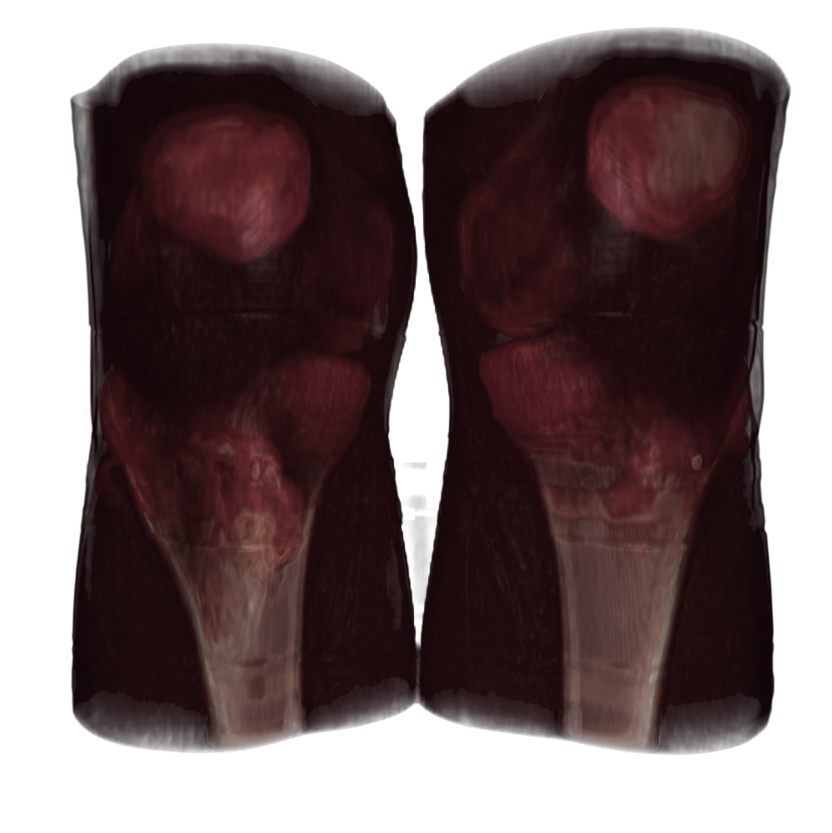
\includegraphics[width=1\linewidth]{CT-Knee_CT-Bone5_even}
			\subcaption{}
		\end{minipage}~
		\begin{minipage}{.3\textwidth}
			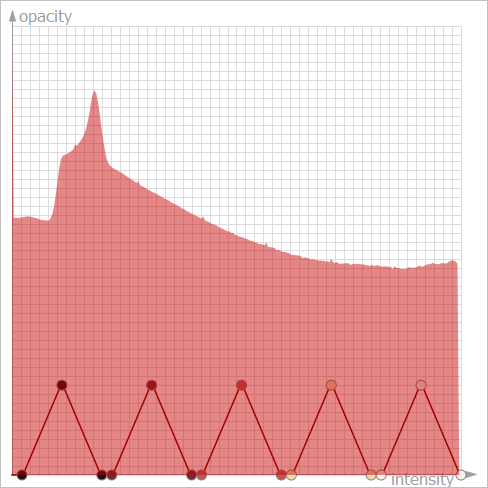
\includegraphics[width=1\linewidth]{tf_CT-Knee_CT-Bone5_even}
			\subcaption{}
		\end{minipage}~
		\begin{minipage}{.4\textwidth}
			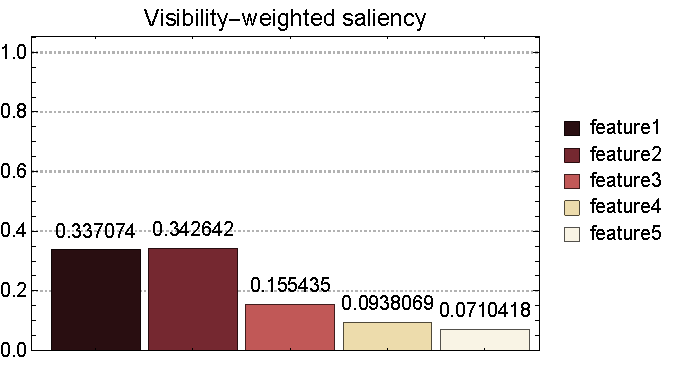
\includegraphics[width=1\linewidth]{CT-Knee_CT-Bone5_even_visibility_saliency_weighted_chart}
			\subcaption{}
		\end{minipage}
		
		\begin{minipage}{.3\textwidth}
			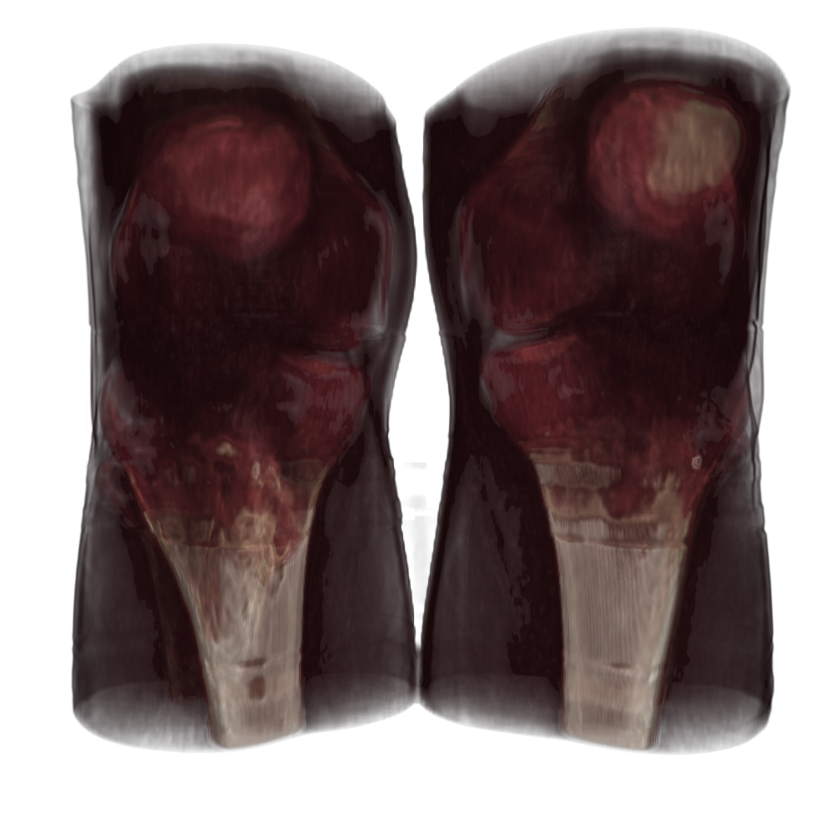
\includegraphics[width=1\linewidth]{CT-Knee_CT-Bone5_even_optimized_parallelsearch_target_even}
			\subcaption{}
		\end{minipage}~
		\begin{minipage}{.3\textwidth}
			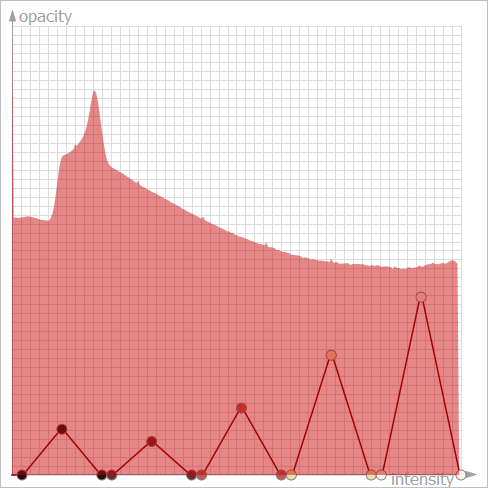
\includegraphics[width=1\linewidth]{tf_CT-Knee_CT-Bone5_even_optimized_parallelsearch_target_even}
			\subcaption{}
		\end{minipage}~
		\begin{minipage}{.4\textwidth}
			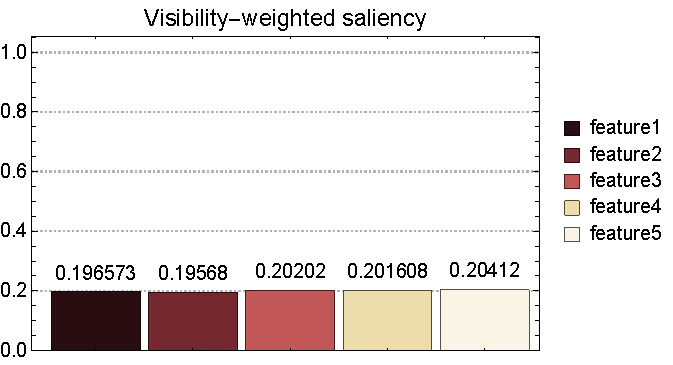
\includegraphics[width=1\linewidth]{CT-Knee_CT-Bone5_even_optimized_parallelsearch_target_even_visibility_saliency_weighted_chart}
			\subcaption{}
		\end{minipage}
		
		\begin{minipage}{.3\textwidth}
			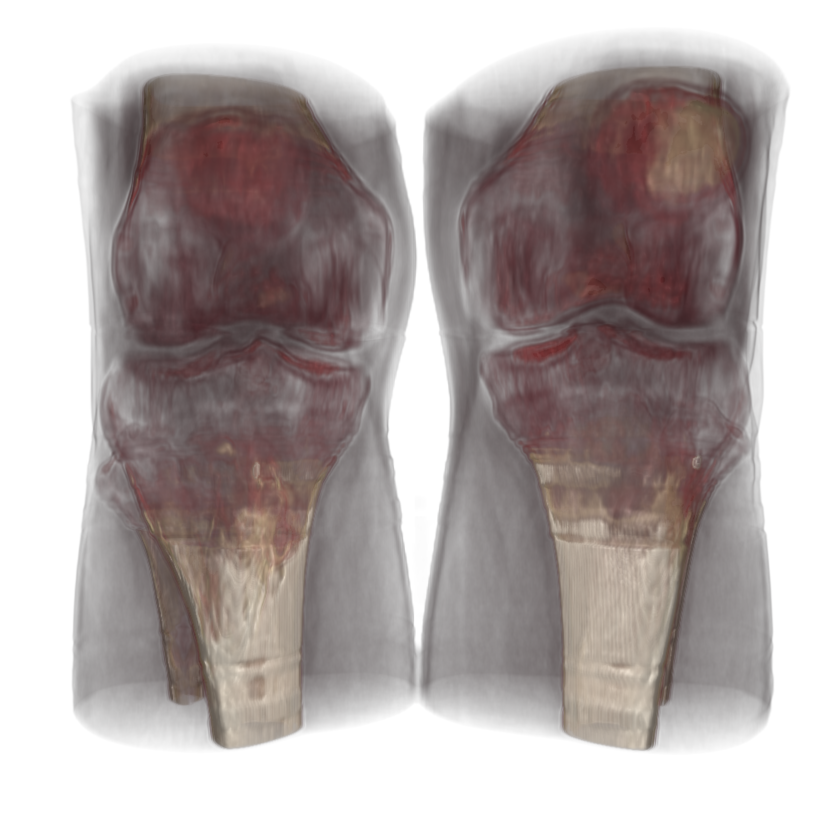
\includegraphics[width=1\linewidth]{CT-Knee_CT-Bone5_even_optimized_parallelsearch_target_diagonal}
			\subcaption{}
		\end{minipage}~
		\begin{minipage}{.3\textwidth}
			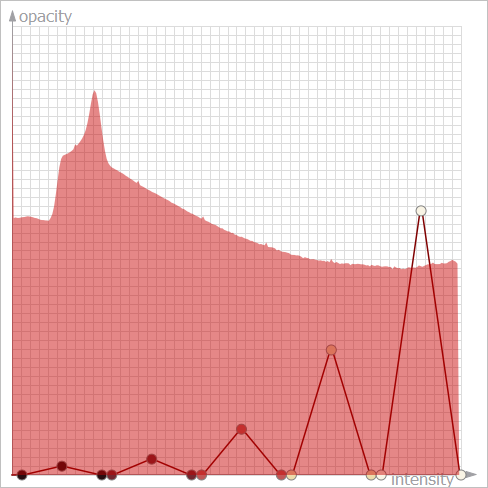
\includegraphics[width=1\linewidth]{tf_CT-Knee_CT-Bone5_even_optimized_parallelsearch_target_diagonal}
			\subcaption{}
		\end{minipage}~
		\begin{minipage}{.4\textwidth}
			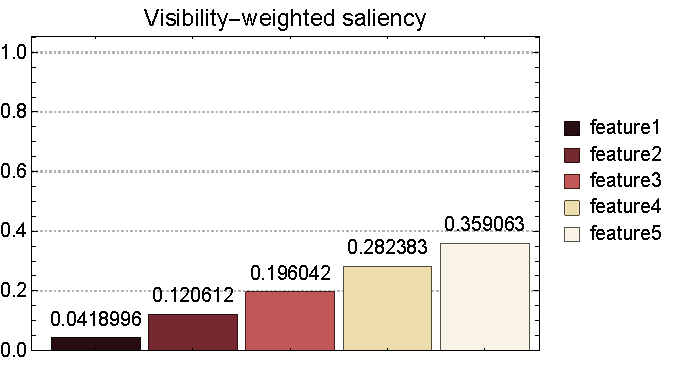
\includegraphics[width=1\linewidth]{CT-Knee_CT-Bone5_even_optimized_parallelsearch_target_diagonal_visibility_saliency_weighted_chart}
			\subcaption{}
		\end{minipage}
	\end{minipage}
	\caption{CT-knee: (a), (b) and (c) are the volume rendered image, transfer function and VWS graph respectively; (d), (e) and (f) are the images after VWS-optimization to a even VWS target, where all features have similar VWS; (g), (h) and (i) are the images after VWS-optimization to a diagonal VWS target, where the internal features are clearer.
		%		(e) Gradient descent with fixed step sizes; (f) Gradient descent with parallel line search
	}
	\label{fig:CT-Knee_CT-Bone5_even}
\end{figure}

\begin{figure}
	\centering
	\begin{minipage}{.9\textwidth}%%%%%%%%%%%%%%%%%%%% ADDED THIS TEMPORARILY AS THIS FIGURE IS OVERFLOWING THE PAGE %%%%%%%%%%
		\begin{minipage}{.3\textwidth}
			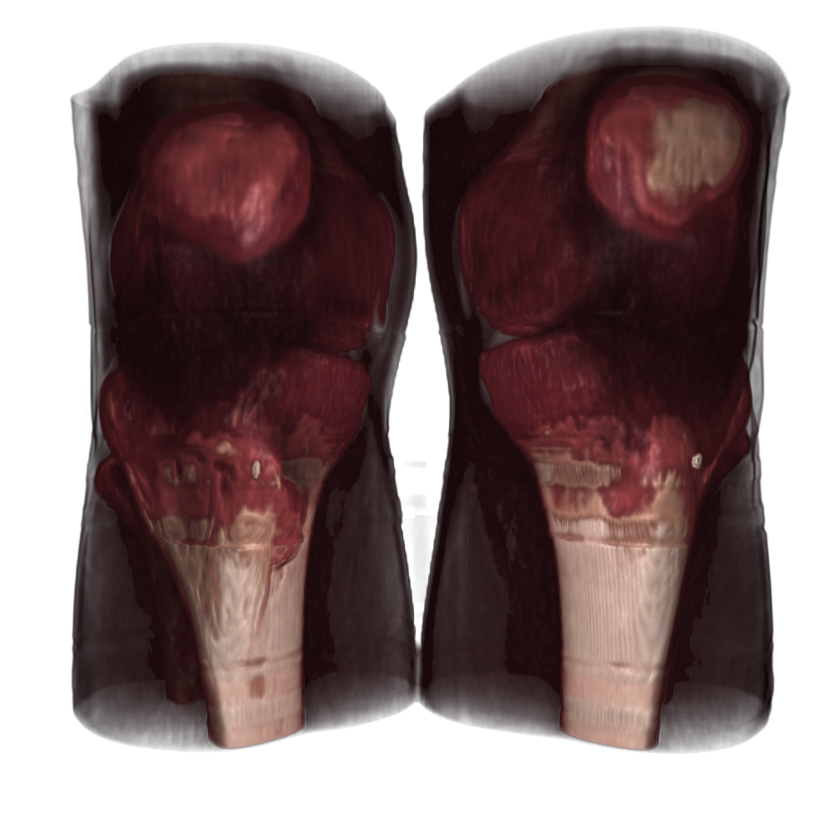
\includegraphics[width=1\linewidth]{CT-Knee_CT-Bone5_diagonal}
			\subcaption{}
		\end{minipage}~
		\begin{minipage}{.3\textwidth}
			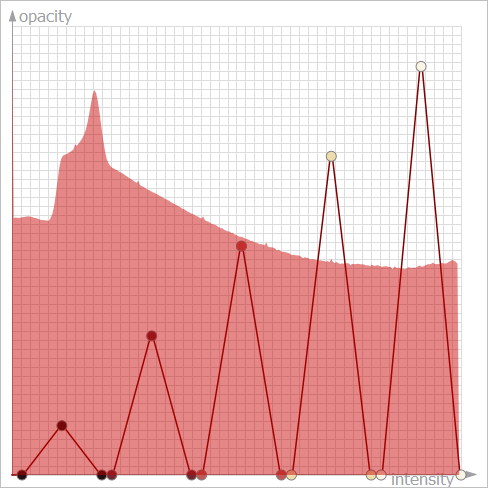
\includegraphics[width=1\linewidth]{tf_CT-Knee_CT-Bone5_diagonal}
			\subcaption{}
		\end{minipage}~
		\begin{minipage}{.4\textwidth}
			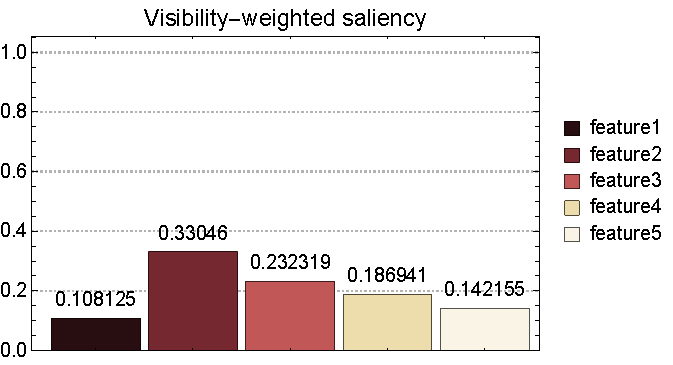
\includegraphics[width=1\linewidth]{CT-Knee_CT-Bone5_diagonal_visibility_saliency_weighted_chart}
			\subcaption{}
		\end{minipage}
		
		\begin{minipage}{.3\textwidth}
			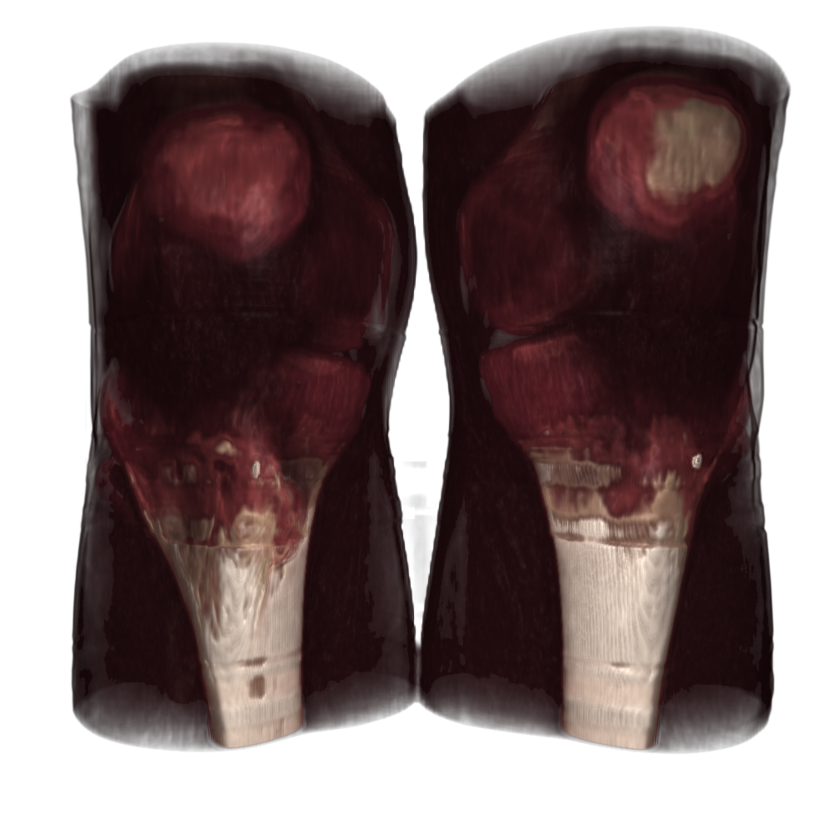
\includegraphics[width=1\linewidth]{CT-Knee_CT-Bone5_diagonal_optimized_parallelsearch_target_even}
			\subcaption{}
		\end{minipage}~
		\begin{minipage}{.3\textwidth}
			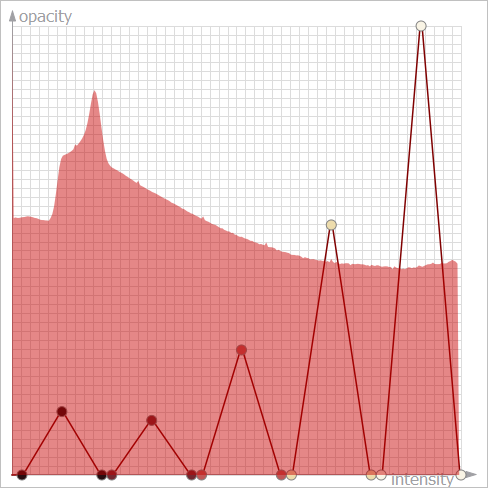
\includegraphics[width=1\linewidth]{tf_CT-Knee_CT-Bone5_diagonal_optimized_parallelsearch_target_even}
			\subcaption{}
		\end{minipage}~
		\begin{minipage}{.4\textwidth}
			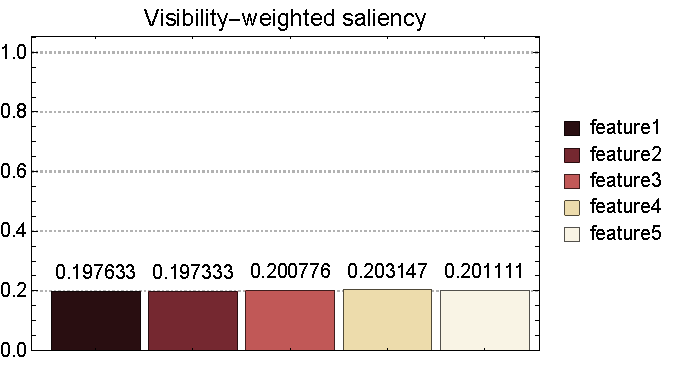
\includegraphics[width=1\linewidth]{CT-Knee_CT-Bone5_diagonal_optimized_parallelsearch_target_even_visibility_saliency_weighted_chart}
			\subcaption{}
		\end{minipage}
		
		\begin{minipage}{.3\textwidth}
			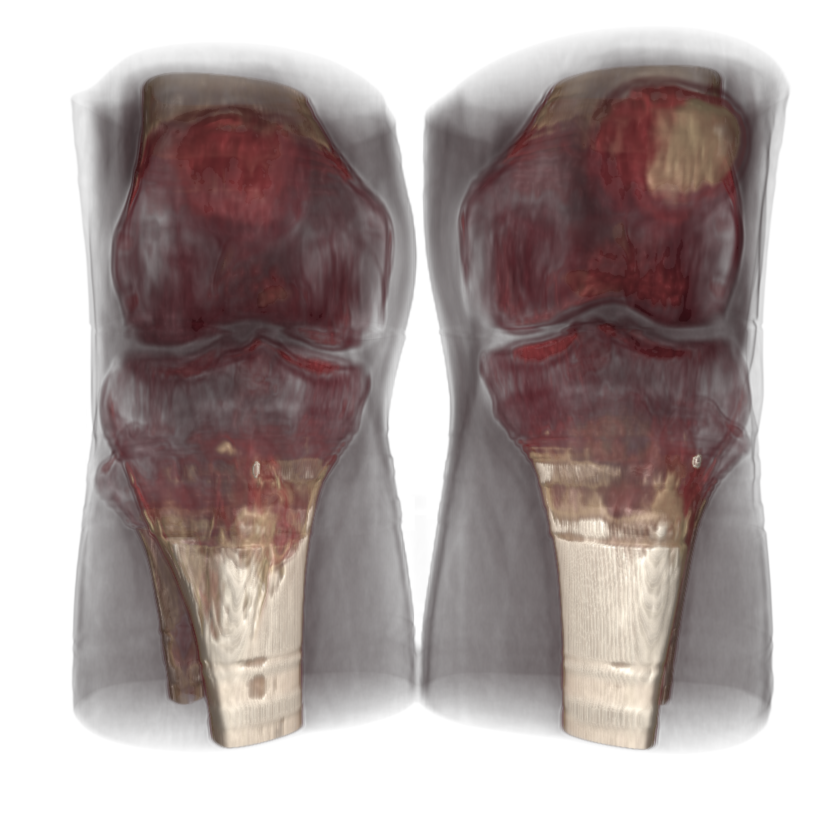
\includegraphics[width=1\linewidth]{CT-Knee_CT-Bone5_diagonal_optimized_parallelsearch_target_diagonal}
			\subcaption{}
		\end{minipage}~
		\begin{minipage}{.3\textwidth}
			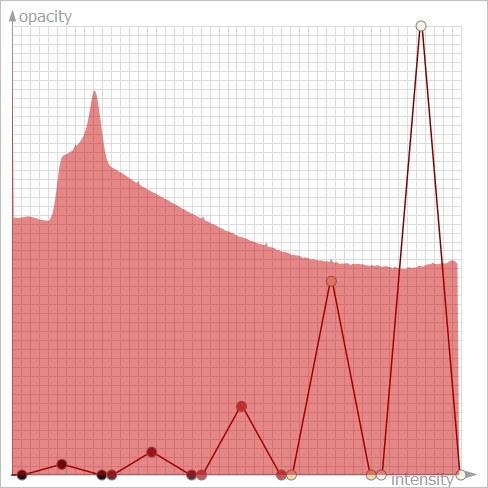
\includegraphics[width=1\linewidth]{tf_CT-Knee_CT-Bone5_diagonal_optimized_parallelsearch_target_diagonal}
			\subcaption{}
		\end{minipage}~
		\begin{minipage}{.4\textwidth}
			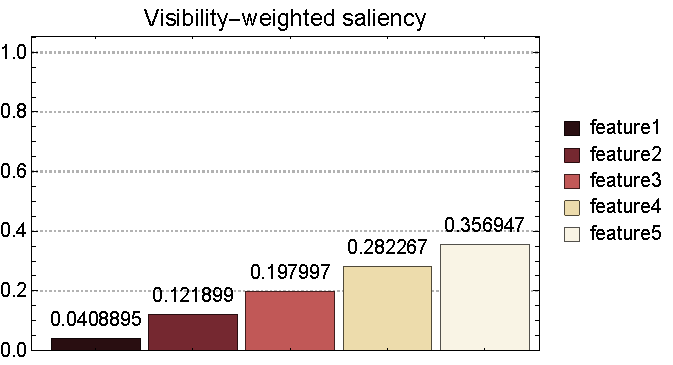
\includegraphics[width=1\linewidth]{CT-Knee_CT-Bone5_diagonal_optimized_parallelsearch_target_diagonal_visibility_saliency_weighted_chart}
			\subcaption{}
		\end{minipage}
	\end{minipage}
	\caption{CT-knee: (a), (b) and (c) are the volume rendered image, transfer function and VWS graph respectively; (d), (e) and (f) are the images after VWS-optimization to a even VWS target, where all features have similar VWS; (g), (h) and (i) are the images after VWS-optimization to a diagonal VWS target, where the internal features are clearer.
		%		(e) Gradient descent with fixed step sizes; (f) Gradient descent with parallel line search
	}
	\label{fig:CT-Knee_CT-Bone5_diagonal}
\end{figure}
